\documentclass{article}
\usepackage{listingsutf8,newtxtt,xcolor,graphicx}
\usepackage[hyphens]{url}
\usepackage{hyperref}
\begin{document}
\title{Übungsblatt 1}
\date{}
\maketitle
\lstset{language=Python,
  basicstyle=\ttfamily,
  keywordstyle=\bfseries\color{magenta},
  stringstyle=\color{red},
  numberstyle=\color{blue}
  breaklines=true,
  showstringspaces=false,
  backgroundcolor=\color{yellow!30},
  ndkeywordstyle=\color{yellow},
  commentstyle=\color{green},
  identifierstyle=\color{black},
  literate=
  {á}{{\'a}}1 {é}{{\'e}}1 {í}{{\'i}}1 {ó}{{\'o}}1 {ú}{{\'u}}1
  {Á}{{\'A}}1 {É}{{\'E}}1 {Í}{{\'I}}1 {Ó}{{\'O}}1 {Ú}{{\'U}}1
  {à}{{\`a}}1 {è}{{\`e}}1 {ì}{{\`i}}1 {ò}{{\`o}}1 {ù}{{\`u}}1
  {À}{{\`A}}1 {È}{{\'E}}1 {Ì}{{\`I}}1 {Ò}{{\`O}}1 {Ù}{{\`U}}1
  {ä}{{\"a}}1 {ë}{{\"e}}1 {ï}{{\"i}}1 {ö}{{\"o}}1 {ü}{{\"u}}1
  {Ä}{{\"A}}1 {Ë}{{\"E}}1 {Ï}{{\"I}}1 {Ö}{{\"O}}1 {Ü}{{\"U}}1
  {â}{{\^a}}1 {ê}{{\^e}}1 {î}{{\^i}}1 {ô}{{\^o}}1 {û}{{\^u}}1
  {Â}{{\^A}}1 {Ê}{{\^E}}1 {Î}{{\^I}}1 {Ô}{{\^O}}1 {Û}{{\^U}}1
  {Ã}{{\~A}}1 {ã}{{\~a}}1 {Õ}{{\~O}}1 {õ}{{\~o}}1
  {œ}{{\oe}}1 {Œ}{{\OE}}1 {æ}{{\ae}}1 {Æ}{{\AE}}1 {ß}{{\ss}}1
  {ű}{{\H{u}}}1 {Ű}{{\H{U}}}1 {ő}{{\H{o}}}1 {Ő}{{\H{O}}}1
  {ç}{{\c c}}1 {Ç}{{\c C}}1 {ø}{{\o}}1 {å}{{\r a}}1 {Å}{{\r A}}1
  {€}{{\euro}}1 {£}{{\pounds}}1 {«}{{\guillemotleft}}1
  {»}{{\guillemotright}}1 {ñ}{{\~n}}1 {Ñ}{{\~N}}1 {¿}{{?`}}1,
  columns=fullflexible,
  keepspaces=true
}
\makeatletter
\def\lst@outputspace{{\ifx\lst@bkgcolor\empty\color{white}\else\lst@bkgcolor\fi\lst@visiblespace}}
\makeatother
\thispagestyle{empty}
\begin{enumerate}
\item Betrachten wir folgendes Python3 Programm:
\lstinputlisting[language=Python]{../../progs/de_AT/1.py}
Tippen Sie dieses Programm unter der Website
\begin{center}\url{https://repl.it/languages/python3}\end{center}
im Fenster \textbf{main.py} ein:
\begin{center}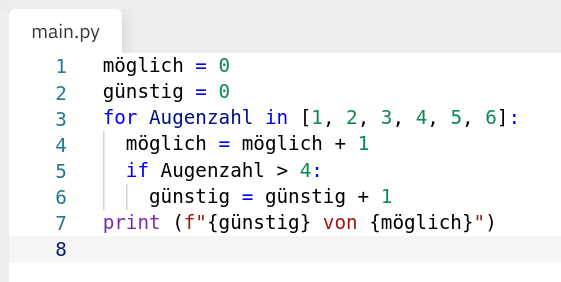
\includegraphics[scale=0.5]{main-py-window}\end{center}
Überprüfen Sie, dass die Einzüge bei Ihnen für jede Zeile genauso aussehen, wie in der Aufgabenstellung.
Sie können den Einzug für jede Zeile am Anfang der Zeile mit der Tab-Taste und mit Shift-Tab kontrollieren.

\item Klicken Sie auf die Run-Taste. Welches Resultat ergibt sich im rechten schwarzen Fenster?

\item Erklären Sie die Bedeutung für jede Zeile des Programms in jeweils einem Satz.

\item Ändern Sie das Programm, so dass das Resultat \texttt{3 von 6} wird.
\end{enumerate}
\end{document}
